\documentclass[french,a4paper,DIV=11,numbers=noendperiod]{scrartcl}

% --- Encodage, langue, fontes ---
\usepackage{iftex}
\ifPDFTeX
  \usepackage[T1]{fontenc}
  \usepackage[utf8]{inputenc}
  \usepackage{lmodern}
  \usepackage[french]{babel}
\else
  \usepackage{fontspec}
  \usepackage{unicode-math}
  \defaultfontfeatures{Scale=MatchLowercase}
  \setmainfont{Latin Modern Roman}
  \setsansfont{Latin Modern Sans}
  \setmonofont{Latin Modern Mono}
  \usepackage[bidi=basic]{babel}
  \babelprovide[main,import]{french}
\fi

% --- Mise en page, microtypographie ---
\usepackage[margin=1.5cm]{geometry}
\usepackage{microtype}
\setlength{\parindent}{0pt}
\setlength{\parskip}{6pt}
\usepackage{ragged2e}
\usepackage[percent]{overpic} % coordonnées en %

% --- Maths ---
\usepackage{amsmath}
\ifPDFTeX
  \usepackage{amssymb}
\fi

% --- Sections non numérotées (style mémo/rapport court) ---
%\setcounter{secnumdepth}{3}

% --- Couleurs, figures, tableaux ---
\usepackage{xcolor}
\usepackage{graphicx}
\usepackage{booktabs,longtable,tabularx,multirow}
\usepackage{float}
\usepackage{caption}
\usepackage{subcaption}

% --- Liens et URLs ---
\usepackage{xurl}
\usepackage{hyperref}
\usepackage[backend=biber,style=authoryear,maxcitenames=2,maxbibnames=99]{biblatex}
\addbibresource{references.bib}

% --- Compat Pandoc/Quarto ---
\providecommand{\tightlist}{\setlength{\itemsep}{0pt}\setlength{\parskip}{0pt}}

% --- Numéros de lignes (optionnel) ---
\usepackage[switch]{lineno}
\linenumbers
\modulolinenumbers[5]

% --- DEBUT ---
\begin{document}
\title{Climatology and trends of extreme precipitation in France: evaluation of an explicit-convection regional climate model}
\author{}
\date{}
\maketitle


\textbf{Authors.}
Nicolas Decoopman, Juliette Blanchet (Univ. Grenoble Alpes, CNRS, INRAE,
IRD, Grenoble INP, IGE, 38000 Grenoble, France), Antoine Blanc (RTM,
ONF, 38000 Grenoble, France).

\textbf{Abstract.} Climate change is intensifying the global water cycle, with extreme precipitation events increasing in frequency and intensity at the global scale. While trends in daily precipitation extremes are well-documented, sub-daily extremes---critical for flash flood risk---remain poorly characterized, due to limited long-term sub-daily observations. Convection-permitting models explicitly resolve deep convection and therefore offer the potential for a substantially improved representation of convective processes and short-duration precipitation extremes. This study evaluates the ability of the convection-permitting regional climate model AROME (2.5 km resolution, 1959--2022), forced by ERA5 reanalysis, to reproduce precipitation extremes and their trends, at daily and hourly scales, using a dense network of Météo-France stations.

Using extreme value theory (GEV modeling), we analyze trends in 10-year return levels for both daily and hourly extremes. At the daily scale, AROME reproduces observed positive trends in southeastern France, consistent with previous studies. Hourly trends are more heterogeneous and less robust, with high spatial variability and low model–observation correlation. Overall, the results highlight the added value of explicit-convection models for extreme precipitation studies while underscoring their limitations for convective extremes.

\textbf{Keywords.} Extreme precipitation, convection-permitting model, AROME, trends, France

\section{Introduction and context}\label{introduction-and-context}

\textbf{Climate change} is driving a warming of the planet's surface
air, with a more pronounced increase over land than over oceans  \parencite{IPCC2021}. Global warming has reached +1.1°C worldwide, +1.7°C in
metropolitan France, and +2°C in the French Alps compared to the
pre-industrial era. Furthermore, the Clausius-Clapeyron relationship
indicates that warmer air can hold more moisture (+7\% per °C)
\parencite{clapeyron1834}. Due to buoyancy (Archimedes' principle), warm air surrounded by cooler air tends to rise. As warm air ascends in the
atmosphere, it undergoes adiabatic cooling, leading to the condensation
of water vapor and the formation of precipitation \parencite{meteofrance}.
However, under calm conditions, the central portion of the precipitation
distribution does not fully capitalize on this excess moisture.
Energetic constraints (radiative balance, evaporation, ocean-air
exchanges) and dynamic constraints (subsidence, synoptic winds) limit
the increase in mean precipitation to only 1--3\% per °C \parencite{IPCC2021}. In
contrast, during intense convective events (thunderstorms, rapid
cyclogenesis), rapid ascent condenses nearly all of this surplus,
causing short-duration extreme rainfall to increase by 5--8\% per
°C---almost matching the theoretical potential. Extreme precipitation
closely follows the Clausius-Clapeyron scaling, whereas mean rainfall
remains influenced by numerous other energetic and dynamic factors
\parencite{ogorman2015contrasting}. Thus, climate warming theoretically leads to an
increase in extreme precipitation, though this increase varies with
changes in atmospheric circulation and can be locally amplified \parencite{blanchet2021explaining}.

\textbf{Extreme precipitation events} are defined as events belonging to the upper tail of the precipitation intensity distribution. There is no consensus
on what constitutes an extreme event. Some authors study
precipitation intensities above the 99th percentile or seasonal/annual
maxima, while others define extreme precipitation as events rarely or
never encountered in a human lifetime (e.g., precipitation levels
expected once every 50, 100 or 10 000 years). Extreme events are at the heart of climate and societal concerns, as they are responsible for numerous casualties and economic costs associated with flooding, landslides, and infrastructure failures \parencite{IPCC_2022_WGIII}.
In 2024, numerous such events made headlines,
including in Nepal, Afghanistan, Central Europe, eastern Spain, and
France \parencite{wmo2024}. Notably, in France in June
2024, intense high-altitude rainfall contributed to major flooding in
the Écrins massif \parencite{Blanc2024}; in October 2024, over 600 mm of
rain in 48 hours caused widespread flooding in the western slopes of the Massif Central
\parencite{MeteoFrance2024_episodesArdeches}; and in May 2025, extremely intense but short-lived
thunderstorms (locally exceeding 120 mm/h) caused extensive damage in
the central Mediterranean region \parencite{MeteoFrance2025}.

\textbf{Daily extremes} have increased in intensity and
frequency across more than half of the world's land regions, at a rate
close to +7\% per °C of warming \parencite{IPCC2021}. Some regional studies
suggest similar trends in a significant proportion of land areas \parencite{Donat2016}. In France, however, signals are far more
heterogeneous and less pronounced than for temperature, with strong
regional variations. In most regions, trends remain weak or
non-significant, and only in certain areas---particularly the
southeast---are signals detected. In this region, the frequency of
extreme Mediterranean episodes (cumulated rainfall \textgreater{} 200 mm
in 24 hours) has doubled between 1961 and 2020, although interannual
variability remains high \parencite{meteofrance2024}. The mean intensity of
daily extremes has increased by +22\% between 1961 and 2015 \parencite{Ribes2019,Blanchet2018,blanchet-creutin-2022}. In southeastern France, no significant trend in annual maxima of daily precipitation was detected before the early 1990s; since then, studies report increases on the order of ~20\% (with estimates reaching ~40\% depending on the metric and uncertainty range) \parencite{Ribes2019}. In the southeastern Alps, the increase in 20-year return
level daily precipitation in autumn (1958--2017) could reach an order of
magnitude comparable to its mean value (\textasciitilde+100\%) \parencite{blanchet2021explaining}. Projections indicate that a +4°C
warming scenario could lead to an average increase of
\textasciitilde+15\% in daily extreme rainfall across France, and up to
+20\% in the northern half \parencite{Soubeyroux01022015}. There remains
strong spatial and interannual variability \parencite{IPCC2021}.

\textbf{Hourly extremes} are
essential for characterizing intense convective phenomena (thunderstorm
downpours, stationary thunderstorms) often responsible for flash floods.
Due to the lack of long, spatially dense time series, there is no
systematic global analysis of sub-daily trends; available data are often
sparse, short, and non-significant. Nevertheless, several regional
studies detect an intensification of hourly extremes across nearly all
continents, though global confidence in an overall increase remains very
low \parencite{IPCC2021}. Increases in extreme rainfall have been observed in the
United States, China (summer), Australia (annually), South Africa
(summer), India, Malaysia, and Italy \parencite{IPCC2021}. Depending on the method and
region, studies highlight sensitivities ranging from +7\% to +13\% per
°C---up to twice the Clausius-Clapeyron rate \parencite{molnar2015relation}. In
France, few regional studies explicitly characterize trends in
hourly extremes. Observed maximum 1-hour values now reach 40--60 mm
during major Mediterranean events, compared to 30--40 mm in the
1980s--1990s \parencite{meteofrance2024}. Only the study by \cite{Berghald2025} quantifies trends in hourly extremes in the French Alps.
However, trends in hourly return levels remain weak to non-significant,
with no clear spatial or seasonal coherence, contrasting with the robust
signals observed at daily time scales \parencite{Soubeyroux01022015}. This suggests that hourly extremes do not yet show a clear climate signal, possibly because the signal is still emerging but cannot be robustly detected given the short length of available series and the high year-to-year variability.

\textbf{In France}, a nationwide network of daily precipitation with good spatial coverage became available from the 1950–1960s, while most hourly records only begin in the 1990–2000s. In parallel, climate models forced by reanalyses provide complementary advantages of: 1) precipitation series that potentially go back further in time than raingauge records; and 2) spatially complete and
physically consistent fields, particularly useful in poorly instrumented
areas. Global Circulation Models (GCMs) are not suitable for studying convective extremes, as convection is parameterized, leading to over-smoothed and
poorly located hourly precipitation at resolutions of 12--200 km \parencite{KilometerScaleClimateModelsProspectsandChallenges}. 
The emergence of regional climate models with convection-permitting offers a unique opportunity, as they realistically simulate the dynamics of intense precipitation at fine spatial and temporal scales over long periods. Recent multi-model convection-premitting ensembles further show that such simulations provide more certain projections of local changes in extreme rainfall, by substantially reducing model-related uncertainty compared to coarser-resolution RCMs \parencite{Fosser2024}. In France, the convection-permitting RCM AROME model (2.5 km) forced by ERA-Interim (1979–2019) has been evaluated by \cite{Caillaud2021,Cortes-Hernandez2024}, who show that AROME realistically reproduces the location, intensity, frequency, and interannual variability of northwestern Mediterranean heavy precipitation events at daily and especially hourly scales, with clear added value compared to the coarser RCM ALADIN. However, the study also reports persistent regional biases, notably an overestimation of rainfall intensity in mountainous areas and an underestimation over coastal plains. These biases are accompanied by timing and spatial-distribution errors in some events, highlighting remaining limitations for the most extreme convective episodes. A new generation of simulation is now available, where AROME is forced by ERA5 (25-31km) from 1959 to 2022. This provides a unique dataset with sufficiently long series (63 years) to study precipitation extremes in France and their trends. However, the validity of the extremes simulated by this model has never been evaluated. Our study
addresses this gap by assessing the ability of the AROME model to reproduce the climatology and trends of daily and hourly precipitation in France.

\section{Data used}\label{data-used}

\subsection{Stations}\label{stations}

In order to evaluate the AROME model, this study uses precipitation data from Météo-France stations
\parencite{meteofrance2024} at daily (1959--2022) and hourly (1990--2022) time
steps. There is a strong contrast between daily and hourly observational records available in France. Daily stations provide long, dense time series: more than half of the 8 198 daily records have over 40 years of data with limited missing values, and several exceed 60 years. In contrast, hourly stations remain much shorter: most of the 2 315 hourly stations offer only 15–30 years of data, reflecting the later deployment of automatic networks. This disparity underscores why long-term trends in sub-daily extremes have been little studied in France so far due to the lack of long records.  
%Figure 1 shows the number of stations maintained by Météo-France as well as the length of the series at different timestep. As illustrated in this figure, there is a strong contrast between daily and hourly observational records available in France. Daily stations (left) provide long, dense time series: more than half of the 8 198 stations have over 40 years of data with limited missing values, and several exceed 60 years. In contrast, hourly stations (right) remain much shorter: most of the 2 315 stations offer only 15–30 years of reliable data, reflecting the later deployment of automatic networks. This disparity underscores why long-term trends in sub-daily extremes are more difficult to detect than at the daily scale. 

Station selection is based on a double criteria: at each station, we compute the proportion of missing data for each year/season/month. A year/season/month is considered as missing if it contains more than 10\% of missing values. Then only the stations with at least the required number of nonmissing years/seasons/months are retained: 50 years for the daily station (1959--2022) and 25 years for hourly stations (1990--2022). Subsequent
analyses are restricted to this subset of stations and years/seasons/months. These criteria, applied over the complete hydrological reference period, lead us to select 1583 daily stations and 574 hourly stations.

\subsection{AROME model}\label{arome-model}

The convection-permitting RCM AROME model, forced by the ERA5 reanalysis, provides
gap-free hourly precipitation data from 1959 to 2022 at a 2.5 km resolution over
the western Europe and northwestern Mediterranean region in Figure \ref{fig:map_domain} (Centre National de
Recherches Météorologiques 2014). This results in 87,536 regularly spaced grid cells over metropolitan France.

\begin{figure}
\begin{center}
  \includegraphics[width=\linewidth]{fig2.pdf}
  %\captionsetup{type=figure}
  %\setcounter{figure}{1}% la prochaine valeur utilisée sera 2
  \caption{Map showing the computational domain of the AROME model. Shading shows topography at 2.5 km resolution and thin lines indicate the 400 m elevation contour. The letters show the geographical zones cited in the article.}\label{fig:map_domain}
\end{center}
\end{figure}

\cite{Caillaud2021} have evaluated the AROME model forced by ERA-Interim. They show a generally good representation of heavy precipitation events, but several systematic biases are documented. The model tends to underestimate the most intense daily and hourly extremes, particularly for the highest values (>200 mm/d and >40 mm/h). AROME also exhibits seasonal temperature biases: a cold bias in winter–spring, and a warm bias in summer associated with an excess of incoming short-wave radiation linked to underestimated cloud cover. In mountainous areas, the model is too cold and too wet, and snow cover tends to persist unrealistically above roughly 2000 m. Some precipitation-system properties (extent, duration, volume) also remain biased when compared with reference products. 

It should be noted that temperature trends with the AROME model forced by ERA5 are twice as weak as observed trends (personnal communication with CNRM researchers). This implies a dampening of the Clausius–Clapeyron–related component of extreme precipitation trends, which is expected to influence the magnitude of the trends we can detect.

\section{Methodology}\label{methodology}

The primary objective of this study is to
validate the AROME model (grid points) against stations
over metropolitan France using precipitation
regime indicators (correlation and bias). This is first conducted under
stationary conditions to focus on the climatology (Section \ref{climatology}), then in a non-stationary context to assess the variability and trends in extremes (Section \ref{trends-in-extremes}).

Evaluation is made per year and season. Seasons are defined as follows: \textbf{OND}:
October (OCT), November (NOV), December (DEC), \textbf{JFM}: January
(JAN), February (FEB), March (MAR), \textbf{AMJ}: April (APR), May
(MAY), June (JUN), \textbf{JAS}: July (JUL), August (AUG), September
(SEP). The hydrological year (\textbf{YEAR}) is defined as the period
from 1 September of year N to 31 August of year N+1.

\subsection{Climatology of extremes}\label{climatology}

%\subsubsection{GEV distribution for extremes}\label{gev-distribution-for-extremes}

While descriptive statistics such as mean precipitation or wet day frequency provide useful summaries for overall precipitation, they cannot assess quality of rare occurrence, e.g. of 10 year return events that are exceeded on average only once every 10 years. %Furthermore, the descriptive statistics of Section 3.1 are stationary, thus they cannot inform about potential trends. 
To address
this limitation, we apply extreme value theory (EVT) \parencite{coles2001introduction}. This states that, under general conditions, the cumulative distribution function (CDF) of block maxima - e.g. annual maxima - can be approximated by the Generalized Extreme Value (GEV)
distribution.

The GEV distribution is a continuous
probability distribution parameterized by the triplet
\(\theta = (\mu, \sigma, \xi)\) --- respectively the location, scale
(strictly positive), and shape---with the following cumulative
distribution function: \[
F(x;\mu ,\sigma ,\xi) = \exp\left\{-\left[1 + \xi\frac{x - \mu}{\sigma}\right]^{-1/\xi}\right\}, \quad 1 + \xi\frac{x - \mu}{\sigma} > 0
\]

It unifies the three classical distributions Gumbel (\(\xi \to 0\)), Fréchet (\(\xi > 0\)) and Weibull (\(\xi < 0\)) where the shape parameter \(\xi\) determines the tail behavior.

The return level (or quantile of order \(1 - \tfrac{1}{T}\)) of the GEV
distribution corresponds to the threshold value exceeded, on
average, once every \(T\) years. 
Denoting by $F^{-1}$ the quantile function of the GEV, it is given by:

\begin{equation}\label{eq:RLstat}
\mathrm{RL}_{T}
= F^{-1}\!\left(1 - \frac{1}{T}\right)
= \mu + \frac{\sigma}{\xi}
\left[
\left(
-\log\!\left(1 - \frac{1}{T}\right)
\right)^{-\xi}
- 1
\right].
\end{equation}


The GEV parameters $(\mu,\sigma,\xi)$ are estimated by maximum likelihood method for each
spatial location separately, considering the block maxima at a given
location to be independent. This gives a set of parameters $\mu,\sigma,\xi$ and thus
return level estimates from Eq.~\ref{eq:RLstat}.

\subsection{Trends in extremes}\label{trends-in-extremes}

\subsubsection{Non-stationary GEV models}\label{non-stationary-gev}

To consider trends in extremes, the GEV distribution can be made non-stationary
by allowing at least one GEV parameter to vary with time: $\mu(t)$, $\sigma(t)$
and/or $\xi(t)$. Owing to the difficulty of estimating the tail parameter $\xi$,
it is assumed stationary, i.e. $\xi(t) = \xi_0$. Three non-stationary models are
considered:

\[
\begin{array}{c@{\qquad}c@{\qquad}c}
% -------- Column 1 --------
\begin{array}{c}
\begin{aligned}
M_1(\theta_1)\\[-0.2ex]
\theta_1 = (\mu_0, \mu_1, \sigma_0, \xi_0)
\end{aligned}\\[0.4ex]
\begin{cases}
\mu(t) = \mu_0 + \mu_1\, t \\
\sigma(t) = \sigma_0 \\
\xi_0
\end{cases}
\end{array}
&
% -------- Column 2 --------
\begin{array}{c}
\begin{aligned}
M_2(\theta_2)\\[-0.2ex]
\theta_2 = (\mu_0, \sigma_0, \sigma_1, \xi_0)
\end{aligned}\\[0.4ex]
\begin{cases}
\mu(t) = \mu_0 \\
\sigma(t) = \sigma_0 + \sigma_1\, t \\
\xi_0
\end{cases}
\end{array}
&
% -------- Column 3 --------
\begin{array}{c}
\begin{aligned}
M_3(\theta_3)\\[-0.2ex]
\theta_3 = (\mu_0, \mu_1, \sigma_0, \sigma_1, \xi_0)
\end{aligned}\\[0.4ex]
\begin{cases}
\mu(t) = \mu_0 + \mu_1\, t \\
\sigma(t) = \sigma_0 + \sigma_1\, t \\
\xi_0
\end{cases}
\end{array}
\end{array}
\]


Furthermore, based on previous studies of trends in extremes in France
\parencite{Blanchet2018,Ribes2019}, we consider the case of a
trend starting at year $t_{+}=1985$, leading to the three models
$M_{1}^{*}$, $M_{2}^{*}$, and $M_{3}^{*}$. For example, in $M_{1}^{*}$:

\[
\mu(t)=
\begin{cases}
\mu_{0} & \text{if } t \le 1985,\\[4pt]
\mu_{0} + \mu_{1}(t-1985) & \text{if } t \ge 1985.
\end{cases}
\]

This gives six non-stationary models, in addition to the stationary model denoted ($M_0$), which corresponds to $\mu(t)=\mu_0$, $\sigma(t)=\sigma_0$, and $\xi(t)=\xi_0$.

\subsubsection{Model selection}\label{model-selection}

For each model, the GEV parameters $\theta$ are estimated by maximum likelihood method for each
spatial location separately. 
At each spatial point, we thus have seven estimated models
\(M_0, M_1, M_2, M_3, M_1^\ast, M_2^\ast\), and \(M_3^\ast\) that we temporarily rename $M_{0}$ to $M_{6}$. We apply for each non-stationary model $M_{j}$, $j \ge 1$, a likelihood ratio test to compare the goodness of fit of $M_{j}$ to that of the stationary model $M_{0}$, accounting for their number of parameters to avoid overfitting. The test is based on computing the statistics $\Lambda_{j}=2\bigl(\ell_{j}-\ell_{0}\bigr)$, where $\ell$ are the maximum likelihood values. Under the null hypothesis that the maxima are stationary, the statistics $\Lambda_{j}$ follows a $\chi^2$ with $k$ degress of freedom, with $k$ equal the difference in the number of parameters between $M_0$ and $M_j$. 

 Let $p_{j}$ be the corresponding $p$-value.  If $p_{j} \le 10\%$, the model $M_{j}$ is considered to perform better than $M_{0}$, otherwise $M_{0}$ is selected. If several models $M_{j}$ are preferred to $M_{0}$, we apply the following procedure: 1) if either $M_{3}$ or $M_{3}^{*}$ are preferred to $M_{0}$, we select among these two models that with the smallest $p$-value among $p_{3}$ and $p_{3}^{*}$; 2) otherwise, we select among $M_{1}$, $M_{1}^{*}$, $M_{2}$, $M_{2}^{*}$ that with the smallest $p$-value among $p_{1}$, $p_{1}^{*}$, $p_{2}$, $p_{2}^{*}$.

This two-step process prioritizes models with simultaneous temporal
effects on \(\mu\) and \(\sigma\) when statistically justified, ensuring
complexity is introduced only when it provides plus-value. In the rest of the article, only the selected model is considered at each location (grid point or station).


\subsubsection{Trend in return level}\label{return-level}

For a non-stationary GEV with parameters $\mu(t)$, $\sigma(t)$ and $\xi_{0}$, the T-year return level is still given by Eq. \ref{eq:RLstat} but it is now a function $RL_T(t)$ of the year $t$.

Owing to the linear form of $\mu(t)$ and $\sigma(t)$ in the considered
non-stationary models, return levels are linear functions of time in
models $M_{1}$, $M_{2}$, and $M_{3}$, and linear only after 1985 in the
breakpoint models $M_{1}^{*}$, $M_{2}^{*}$, and $M_{3}^{*}$. In the
stationary model $M_{0}$, return levels are of course constant over time.
For the non-stationary models, the relative trend in the $T$-year return
level (\%) over the most recent 30-year period (between 1992 and 2022) is computed as

\[
\mathrm{RelTrend} =
\frac{\mathrm{RL}_{T}(2022)-\mathrm{RL}_{T}(1992)}
{\mathrm{RL}_{T}(1992)}.
\]

It is obviously $0$ if the stationary model has been selected.

\subsubsection{Confidence intervals for the return levels}\label{maximu-likelihood-estimation-and-confidence-intervales}

Noting that the
$T$-year return level function can be written as
$\mathrm{RL}_{T}(t)=\mathrm{RL}_{T,0}+\mathrm{RL}_{T,1}\, t$
for models $M_{1}$, $M_{2}$, $M_{3}$ and
\[
\mathrm{RL}_{T}(t)=
\begin{cases}
\mathrm{RL}_{T,0} & \text{if } t<1985,\\[4pt]
\mathrm{RL}_{T,0}+\mathrm{RL}_{T,1}(t-1985) & \text{if } t>1985,
\end{cases}
\]
for models $M_{1}^{*}$, $M_{2}^{*}$, $M_{3}^{*}$,
confidence intervals for the trend coefficient $\mathrm{RL}_{T,1}$ are obtained
by profiling the likelihood with respect to $\mathrm{RL}_{T,1}$ \parencite{coles2001introduction}. If
the $90\%$ confidence interval of $\mathrm{RL}_{T,1}$ does not contain $0$, the
$T$-year return level trend is not significant at level $10\%$.



%\subsection{Assessing the agreement between AROME and the stations}\label{assessing}
%
%We evaluate the agreement between each
%Météo-France station is matched to the corresponding AROME grid point
%(2.5 km × 2.5 km) based on its spatial location. This
%correspondence allows calculating the Pearson correlation (\(r\)) and
%mean error (\(ME\)) between observed and simulated statistics.

\section{Results}\label{results}

We begin by evaluating, grid point by grid point, the ability of AROME
to reproduce the precipitation regime observed by Météo-France stations.
This initial stationary evaluation allows assessing the quality of the extreme-value climatology before examining return-level trends.

\subsection{Evaluation of the precipitation climatology of AROME}
\label{evaluation-of-the-precipitation-climatology-by-arome}

Figure~\ref{fig:map_clim} provides a spatial comparison of the precipitation climatology between AROME and Météo-France stations. In addition to the 10-year return level assessing quality of extremes, we show two descriptive statistics assessing the overall climatology of precipitation: the mean number of wet days per year (precipitation exceeding 1 mm) and the mean annual total precipitation. Across all indicators, AROME reproduces the large-scale spatial structures with high spatial correlations: Pearson correlation \emph{r} = 0.95 for the annual frequency of precipitation days, \emph{r} = 0.94 for annual cumulative precipitation, \emph{r} = 0.95 for the daily 10-year return level, and a lower correlation of \emph{r} = 0.78 for the hourly 10-year return level. The model correctly captures the main climatic gradients of France: dryness of the Rhône valley and the Mediterranean coast,(50-70 wet days per year, annual totals no more than 550 mm per year) contrasting with the wetness of the mountain ranges (Alps, Pyrenees, Massif Central, Vosges, Jura; 140--160 wet days per year, annual totals up to more than 1800 mm per year). The model also reproduces the localization of the largest extremes along the Massif Central ridge and to a lesser extent in the Rhône valley and along the Mediterranean coast at both daily and hourly scales.

\begin{figure}[htbp]
    \centering
    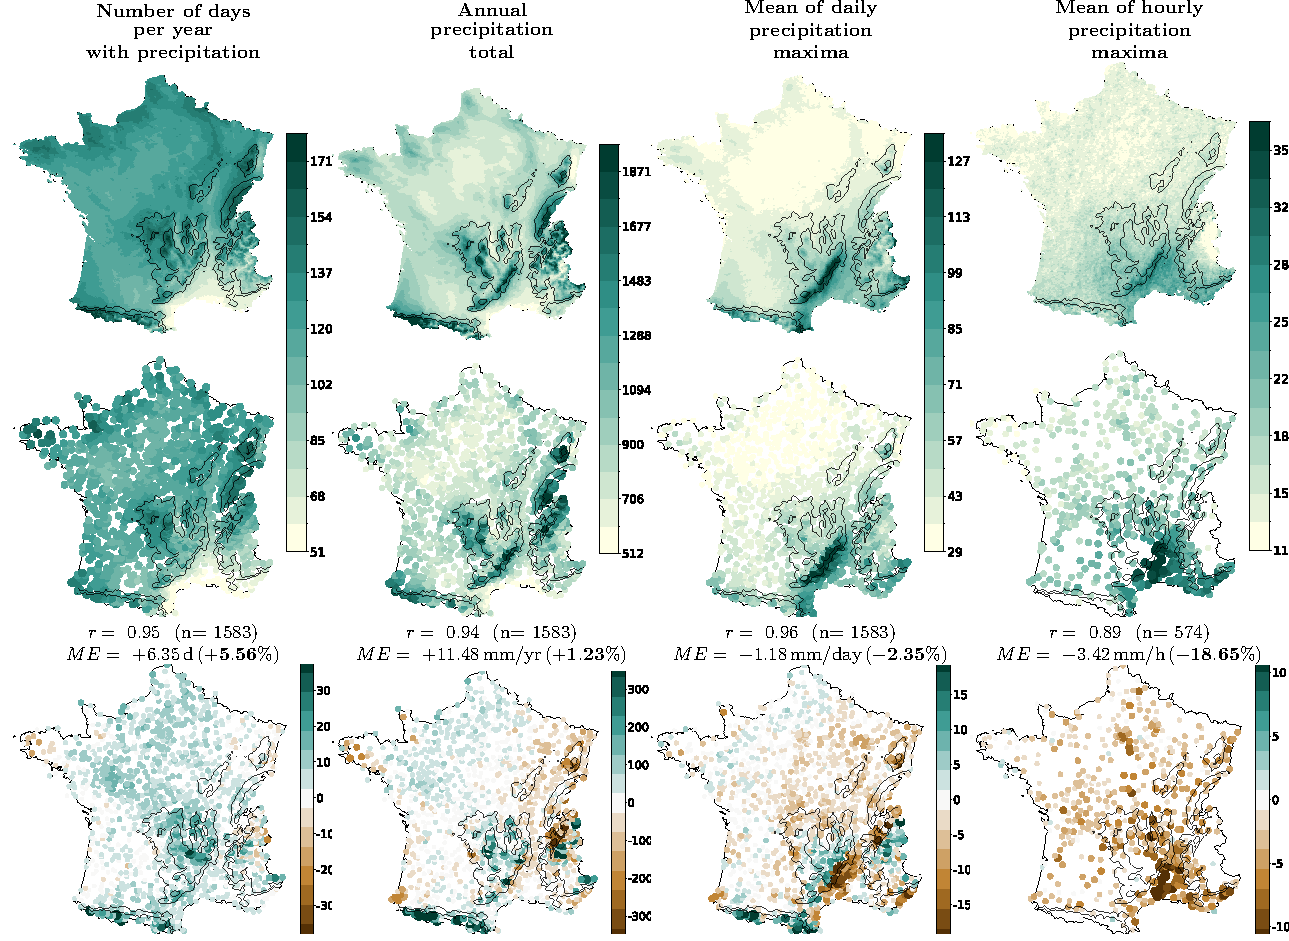
\includegraphics[width=\textwidth]{fig3.pdf}
    %\setcounter{figure}{2}
    \caption{Climatology between the AROME model (first row), Météo-France stations (second row) with the correlation ($r$) and the number of stations compared (n), and the AROME–Station difference (third row) with the bias ($ME$) and the associated relative deviation (\%) derived from daily data from 1959 to 2022 and hourly data from 1990 to 2022 for a hydrological year. The contour lines show the 400 and 800 m isolines. To ease visualization, colour scales are symmetrically saturated. Depending on the statistic, we apply a saturation threshold (99.9\% for the number of days and 99\% for annual and 10-year return level precipitation). All maps are clipped to this common percentile range.}\label{fig:map_clim}
\end{figure}

Despite this overall agreement, the difference maps reveal structured regional biases. For precipitation frequency, AROME shows little mean bias (+6 days/year) but local excesses above +30 days/year in the Massif Central and Pyrenees, while negative biases (-10 to -30 days/year) appear in the Northern Alps, Brittany, and the Vosges. For annual cumulative precipitation, the mean bias is very small (+11 mm/year) but regional discrepancies reach more than +300 mm per year along the Pyrenean ridge and Northern Alps, and -100 to -400 mm per year from the Northern Pré-Alps to the Vosges. For daily 10-year return level, AROME shows almost no mean bias (-2 mm) but it spreads the extremes too widely around the Massif Central ridge, giving local deficits of -10 to -20 mm along the ridge where the station extremes are the largest and +10 - +30 mm over the Massif Central Plateau. Overestimation is also visible in Northern Alps and the Pyrenees.  At the hourly scale, AROME strongly underestimates the 10-year return levels (\(-6.37\) mm, \(-23.30\)\,\%), with widespread deficits \(-5\) to \(-20\) mm over most of France, especially the southern Massif Central and the Rhône Valley.

The good performance of AROME for the frequency of wet days, the annual precipitation and the daily extremes is found across all seasons (see Figure \ref{fig:correlation_clim}), despite a slight loss in performance in spring and summer for the extremes (AMJ to JAS, correlation around $0.9$). Performance is lower for hourly extremes across all seasons and particularly in spring where correlation drops to 0.38.

%\paragraph{Correlation analysis (Figure~4).}
%Each Météo-France station is matched to its nearest AROME grid point (2.5~km~$\times$~2.5~km), which enables the computation of the Pearson correlation (\emph{r}) between observed and simulated values. Regardless of the indicator (Figure~4), the AROME model faithfully reproduces the station-based statistics, with correlations never falling below 0.38.

%Irrespective of the temporal scale---daily (1959--2022 or 1990--2022) or hourly (1990--2022)---and the season, the agreement between AROME and the raingauge data is very strong for the number of rainy days and for cumulative precipitation. As shown in the first two panels of Figure~4, correlations systematically reach 0.92--0.98 for \textbf{YEAR}, \textbf{OND}, \textbf{JFM}, \textbf{AMJ} and \textbf{JAS}. This high performance is maintained for the 10-year return level of daily precipitation (\textbf{YEAR}, \textbf{OND}, \textbf{JFM}, \textbf{AMJ}), but decreases in summer (\textbf{JAS}), where the correlation drops to 0.90.

%The degradation is more pronounced at the hourly scale. Correlation decreases by up to 0.5 points compared with the daily estimates, falling to 0.78--0.88 (\textbf{YEAR}, \textbf{OND}, \textbf{JFM}, \textbf{AMJ}), and to 0.38 in summer (\textbf{JAS}). This reflects AROME’s tendency to under-represent convective extremes during the warm season, despite a well-captured spatial structure.

\begin{figure}[htp]
\centering
    \includegraphics[width=0.85\textwidth]{fig4.pdf}
    %\captionsetup{type=figure}
    %\setcounter{figure}{3}% prochaine légende = Figure 4
    \caption{Correlations of climatological indices between the AROME model and Météo-France stations at daily and hourly scales.}\label{fig:correlation_clim}
\end{figure}

\subsection{Evaluation of extreme precipitation
trends}\label{evaluation-of-extreme-precipitation-trends}

\subsubsection{Daily}

At the daily scale, station-based trends in the 10-year return level (Figure~\ref{fig:map_daily_trend}) show spatially coherent but region-dependent signals across France over 1959--2022. For the hydrological year (YEAR), trends are predominantly positive, with a clear reinforcement along the Rhône Valley (+5\% to \(>+30\%\)) and in the southern Alps (+20\% to +30\%). Elsewhere, trends are weak, of mixed sign, and often not significant, supporting a seasonal breakdown. Autumn (OND) shows a similar pattern in trends as the annual scale, with the exception of the Paris area that shows a decrease (-5 to -20\%). In winter (JFM), France is cut in three with a diagonal of decrease from the Mediterranean coast to the Atlantic coast (-10 to -40\%) and mainly increases elsewhere. Spring (AMJ) is characterized by a more spatially uniform positive trend over much of the country, with local increases exceeding +35\%. Ssummer (JAS), shows predominantly negative trends in the southern half of France, apart in the Rhône valley, with an accentuated decrease along the Mediterranean coast (up to -40\%) and mainly positive trends in the northern half.

AROME reproduces the broad spatial organization of these daily-scale patterns but generally underestimates their amplitudes. For the hydrological year, the model captures the significant increase in the Southern Alps, albeit with weaker intensities, and does not reproduces the Rhône Valley reinforcement observed in the stations. Autumn is the season when trends are best represented. AROME correctly identifies the negative anomalies in northern and western France and the positive signal in the Rhône valley and southern Alps, but it underestimates the strength of decreases in the northern Alps. In winter, the model retrieves the north-negative / northeast-positive configuration but all trends are less marked and it misses the decrease over the Alps. In spring, AROME produces weak and poorly organized signals and fails to reproduce the widespread positive trends measured by the stations. In summer, the model correctly identifies a general negative tendency over the souther half of France but he does not see the increase over the Rhône valley and the northern half of France. These discrepancies are consistent with the seasonal performance metrics, which show low correlations and mean biases ranging from $ME = -0.52\%$ (winter) to $ME = -6.24\%$ (spring). Overall, AROME captures the large-scale signs and structure of daily return-level trends but tends to underestimate both their intensity and spatial coherence.

\begin{figure}[htbp]
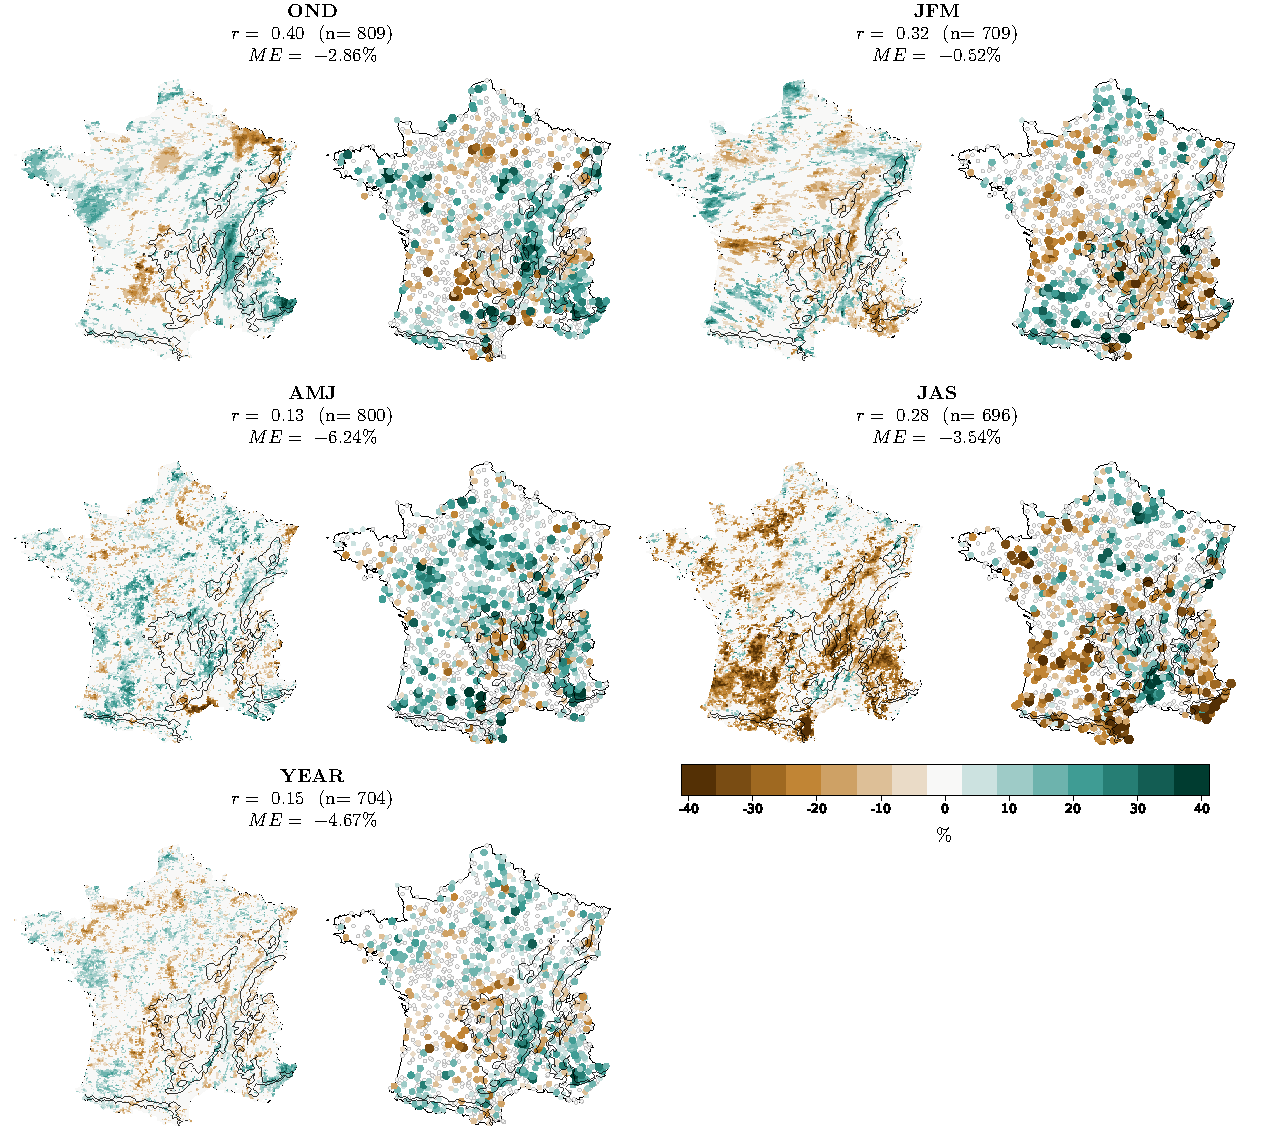
\includegraphics[width=0.85\textwidth]{fig5.pdf}
\caption{Relative trends over the last thirty years ending in 2022 (\%) in the 10-year return level of daily precipitation for AROME (left) and Météo-France stations (right), with the correlation ($r$), the number of stations compared (n), and the bias ($ME$). These results are derived by fitting, at each location, the selected GEV model to daily precipitation maxima from 1959 to 2022. The contour lines show the 400 and 800 m isolines. To ease visualization, colour scales are symmetrically saturated using a 99\% threshold. All maps are clipped to this common percentile range. Only statistically significant trends are shown, non-significant trends are set to zero.}\label{fig:map_daily_trend}
%  \centering
%  \nolinenumbers
%  %\setcounter{figure}{5}
%  \begin{overpic}[width=\linewidth]{fig5.pdf}
%    % Ajuster 73,6 (x,y en %) et la largeur 0.25\linewidth
%    \put(53,8){%
%      \colorbox{white}{%
%        \parbox{0.42\linewidth}{\justifying\footnotesize
%          {\figurename~\thefigure} — Relative trends over the last thirty years ending in 2022 (\%) in the 10-year return level of daily precipitation for AROME (left) and Météo-France stations (right), with the correlation ($r$), the number of stations compared (n), and the bias ($ME$). These results are derived by fitting, at each location, the selected GEV model to daily precipitation maxima from 1959 to 2022. The contour lines show the 400 and 800 m isolines. To ease visualization, colour scales are symmetrically saturated using a 99\% threshold. All maps are clipped to this common percentile range. Only statistically significant trends are shown, non-significant trends are set to zero.%
%        }%
%      }%
%    }
%  \end{overpic}
  % évite une seconde légende visible mais garde la cohérence des flottants
%  \captionsetup{labelformat=empty}
%  \caption{}\label{fig:map_daily_trend}
\end{figure}
%\linenumbers

\subsubsection{Hourly}

At the hourly scale (Figure~\ref{fig:map_hourly_trend}), station-based trends in the 10-year return level over 1990--2022 are markedly more heterogeneous, noisy, and locally more extreme than their daily counterparts (Figure~\ref{fig:map_daily_trend}), with significant trends ranging $[-50\%, +100\%]$ versus $[-30\%, +30\%]$ at the daily scale. Most of the significant trends are highly positive although often isolated.  Over the hydrological year, almost no trend is found apart in few isolated stations where trends reach $\pm 50\%$ and occasionally exceed $+100\%$. Seasonally, the signals remain highly contrasted. In autumn, a pronounced positive pattern emerges along the Mediterranean coast, locally approaching $+100\%$. In winter, intense increases of $+80\%$ to $+100\%$ are found over western France, the eastern Pyrenees, and the Rhône Valley. Spring is the only season when a quite coherent pattern is found. Stations exhibit widespread and very strong increases across much of the country, frequently above $+60\%$ and locally approaching $+100\%$. In summer, spatial variability reaches its maximum, with trends spanning the full range from $-100\%$ to $+100\%$, particularly in the Rhône Valley. These patterns reflect both the strong local variability of convective extremes and the limited length of the hourly record, which jointly hinder the emergence of a clear regional-scale climate signal.

AROME only partially reproduces these hourly-scale patterns. Across all seasons, the model simulates weak and spatially inconsistent signals and fails to capture the most pronounced positive trends seen in the station data. For the hydrological year, spatial correlation between AROME and stations remains low ($r \approx 0.12$), and seasonal correlations are close to zero for several seasons. Mean biases are substantial and of varying sign, with values reaching $ME = +84.7\%$ in spring and $ME = -28.4\%$ in summer. While AROME occasionally recovers the sign of the observed trends in some regions, it generally does not reproduce their fine-scale spatial organization or amplitude. 

\begin{figure}[htbp]
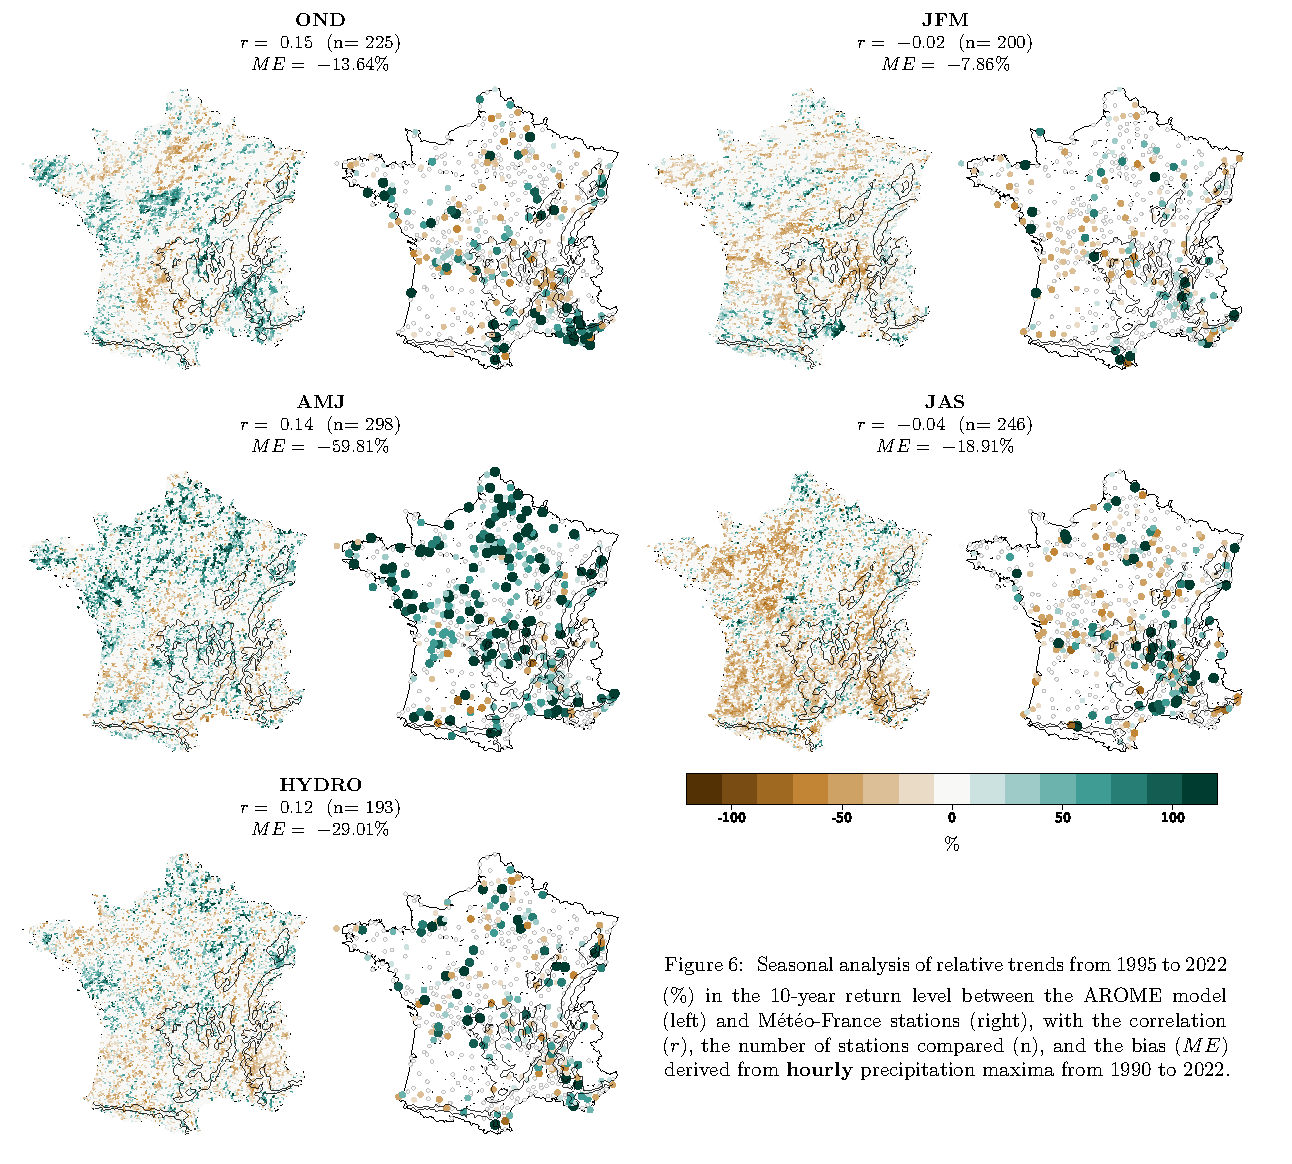
\includegraphics[width=0.85\textwidth]{fig6.pdf}
\caption{Relative trends over the last thirty years ending in 2022 (\%) in the 10-year return level of hourly precipitation for AROME (left) and Météo-France stations (right), with the correlation ($r$), the number of stations compared (n), and the bias ($ME$). These results are derived by fitting, at each location, the selected GEV model to hourly precipitation maxima from 1990 to 2022. The contour lines show the 400 and 800 m isolines. To ease visualization, colour scales are symmetrically saturated using a 90\% threshold. All maps are clipped to this common percentile range. Only statistically significant trends are shown, non-significant trends are set to zero.}\label{fig:map_hourly_trend}
%  \centering
%  \nolinenumbers
%  %\setcounter{figure}{6}
%  \begin{overpic}[width=\linewidth]{fig6.pdf}
%    % Ajuster 73,6 (x,y en %) et la largeur 0.25\linewidth
%    \put(53,8){%
%      \colorbox{white}{%
%        \parbox{0.42\linewidth}{\justifying\footnotesize
%          {\figurename~\thefigure} — Relative trends over the last thirty years ending in 2022 (\%) in the 10-year return level of hourly precipitation for AROME (left) and Météo-France stations (right), with the correlation ($r$), the number of stations compared (n), and the bias ($ME$). These results are derived by fitting, at each location, the selected GEV model to hourly precipitation maxima from 1990 to 2022. The contour lines show the 400 and 800 m isolines. To ease visualization, colour scales are symmetrically saturated using a 90\% threshold. All maps are clipped to this common percentile range. Only statistically significant trends are shown, non-significant trends are set to zero.%
%        }%
%      }%
%    }
%  \end{overpic}
%  % évite une seconde légende visible mais garde la cohérence des flottants
%  \captionsetup{labelformat=empty}
%  \caption{}%
\end{figure}
%\linenumbers

%\subsubsection{Monthly refinement}

%\paragraph{Spatial representation (Figure~7).} 
The monthly analysis (Figure~\ref{fig:map_monthly_trend}) further highlights the specificity of convective regimes and the strong temporal concentration of some signals. Station data show that hourly 10-year return level trends are not uniformly distributed throughout the year but cluster in a few key months. In late winter, strong increases emerge over the Rhône Valley and the Mediterranean coast in February, while March extends these trends all along the western Mediterranean arc. In late autumn, November exhibits substantial increases on the eastern Mediterranean coast (Azur region). In early summer, June displays the clearest signal with widespread positive trends over almost all of France, with local values exceeding $+150\%$. 

AROME reproduces partly the enhanced activity of some months but it underestimates their magnitude and misplaces some of the spatial structures. The model reproduces the existence of positive signals in February, March, November, and June, consistent with the station-based identification of convectively active months. However, the simulated trends are often weaker by a factor of two and display inconsistent spatial localization compared with observations, as reflected by very low spatial correlations for some months (e.g.\ $r = 0.08$ in June).

\begin{figure}[htp]
\centering
    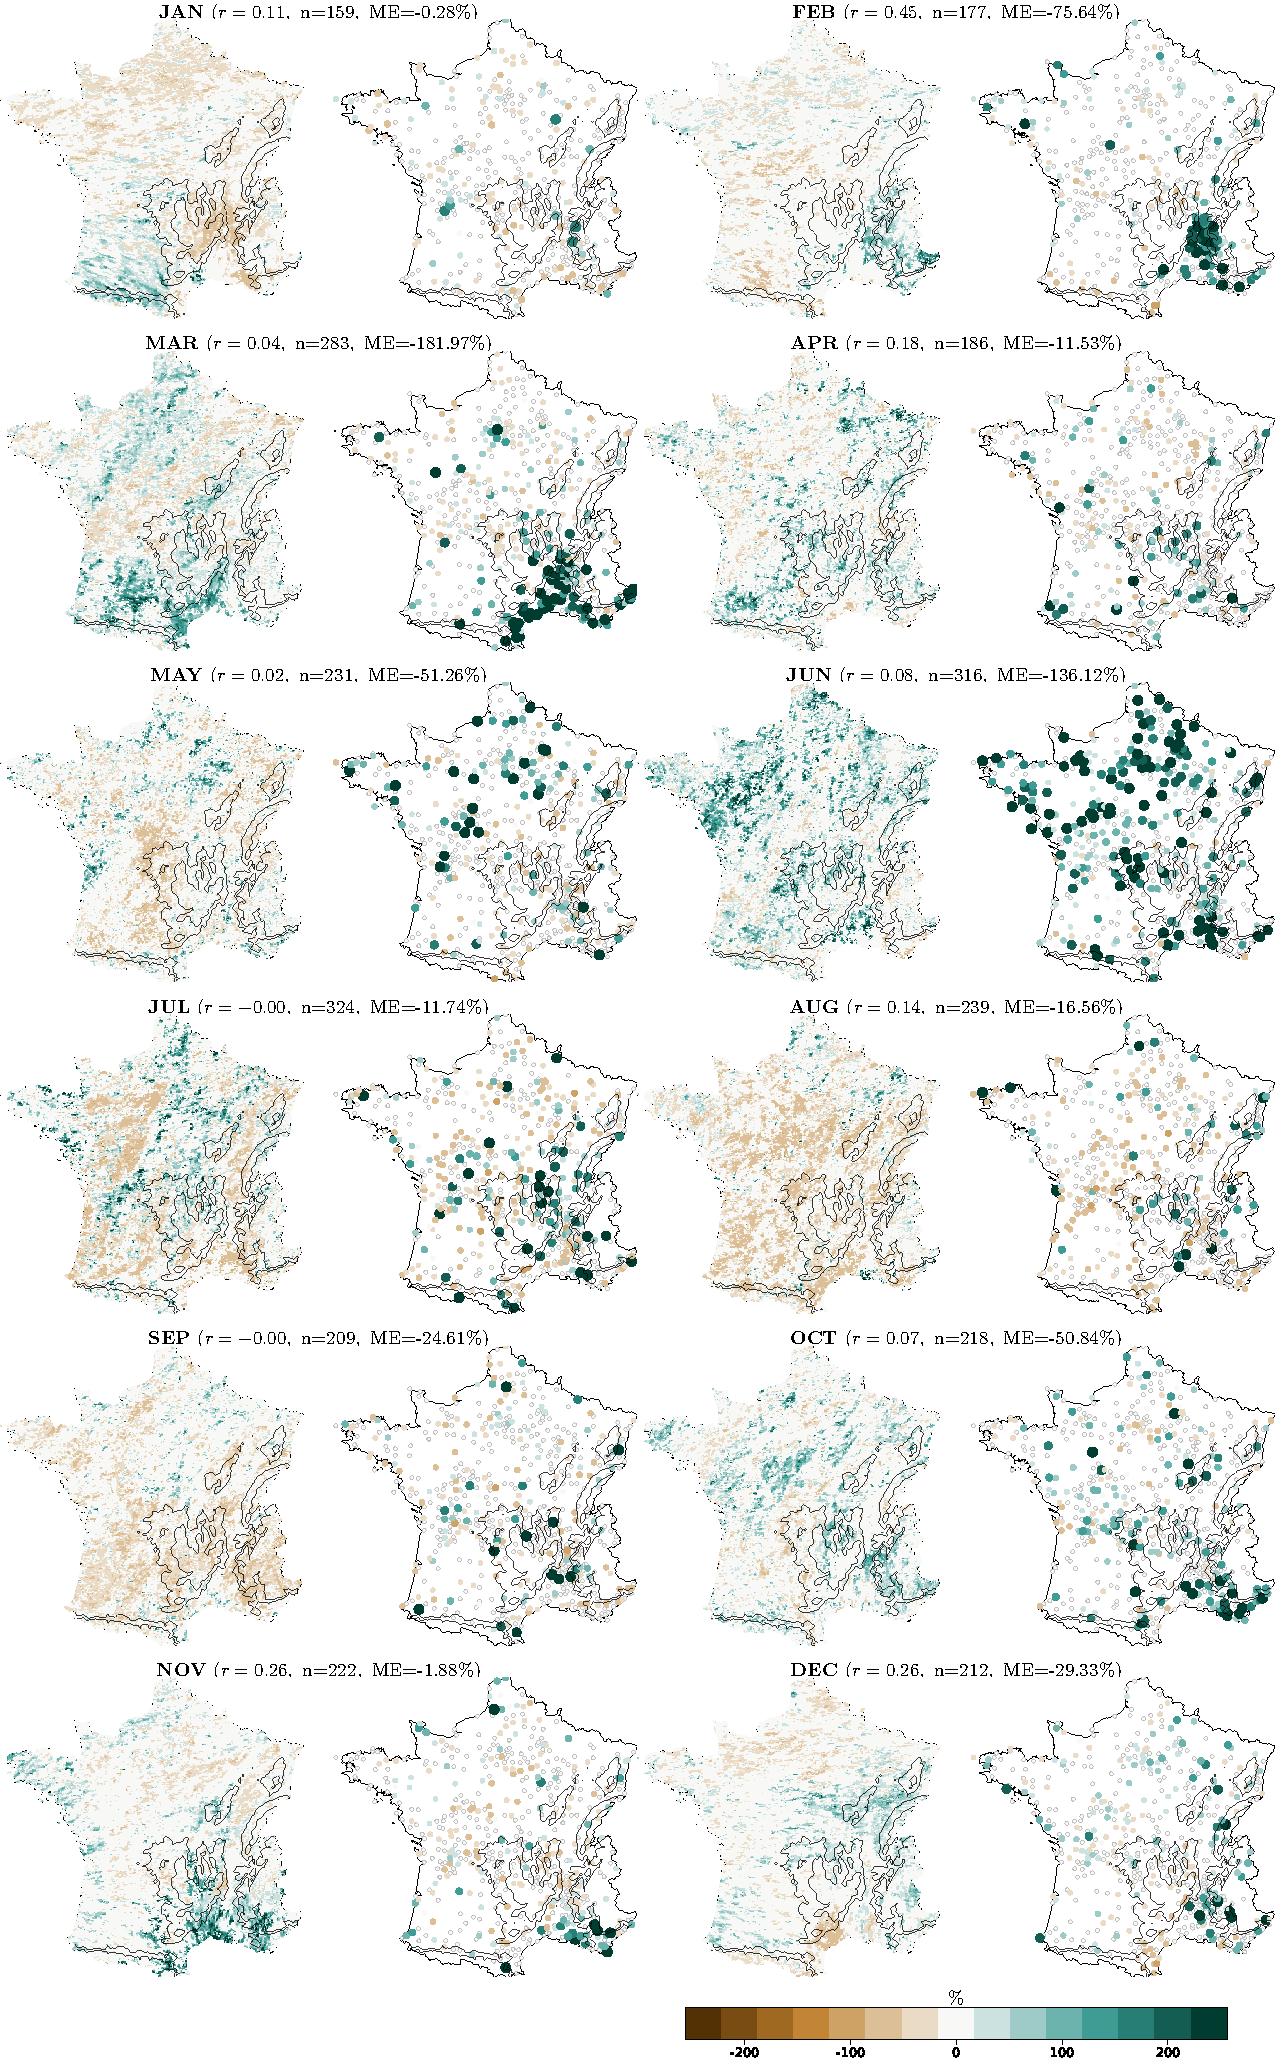
\includegraphics[width=0.80\textwidth]{fig7.pdf}
    %\setcounter{figure}{6}% prochaine légende = Figure 7
    \caption{
        Relative trends over the last thirty years ending in 2022 (\%) in the 10-year return level of hourly precipitation for AROME (left) and Météo-France stations (right), with the correlation ($r$), the number of stations compared (n), and the bias ($ME$). These results are derived by fitting, at each location, the selected GEV model to daily precipitation maxima from 1990 to 2022. The contour lines show the 400 and 800 m isolines. To ease visualization, colour scales are symmetrically saturated using a 90\% threshold. All maps are clipped to this common percentile range. Only statistically significant trends are shown, non-significant trends are set to zero.
        }\label{fig:map_monthly_trend}
\end{figure}

%\paragraph{Correlation analysis (Figure~8).} 
Figure~\ref{fig:correlation_trend} summarizes the spatial correlations between AROME and station-based monthly trends, confirming an overall better representation at the daily than at the hourly scale, with strong month-to-month variability. At the daily scale (1959–2022), correlations span from 0.07 to 0.62 depending on the month, peaking in early winter (December: 0.616; January: 0.569; November: 0.557) and remaining high in late summer (August: 0.512) and early spring (March: 0.526). Agreement weakens markedly in spring and early summer, with correlations dropping to 0.193 in April and reaching a minimum of 0.070 in June. Hourly trends (1990–2022) are generally lower and less consistent, ranging from −0.004 to 0.445: correlations exceed 0.25 only in February (0.445), November (0.256), and December (0.258), while they remain near zero in March (0.039) and May (0.022) and become negligible in September (−0.004). Overall, these results indicate that AROME captures part of the large-scale structure of monthly trend patterns—more clearly at the daily scale—whereas its representation at the hourly scale remains limited, consistent with the stronger local and convective variability affecting sub-daily extremes.

\begin{figure}[htp]
\centering
    \includegraphics[width=\textwidth]{fig8.pdf}
    %\captionsetup{type=figure}
    %\setcounter{figure}{7}% prochaine légende = Figure 7
    \caption{Correlations of relative significant trends between AROME and Météo-France stations, by month.
Values above each bar indicate the number of stations used in the calculation.}\label{fig:correlation_trend}
\end{figure}

%\begin{figure}[htbp]
%    \centering
%    \includegraphics[width=\textwidth]{fig_AROME_trend_saisons.pdf}
%    \\
%    \small FIGURE Y - Tendances horaires d'AROME sur la période 1959--2022 par saison.
%\end{figure}

%\begin{figure}[htbp]
%    \centering
%    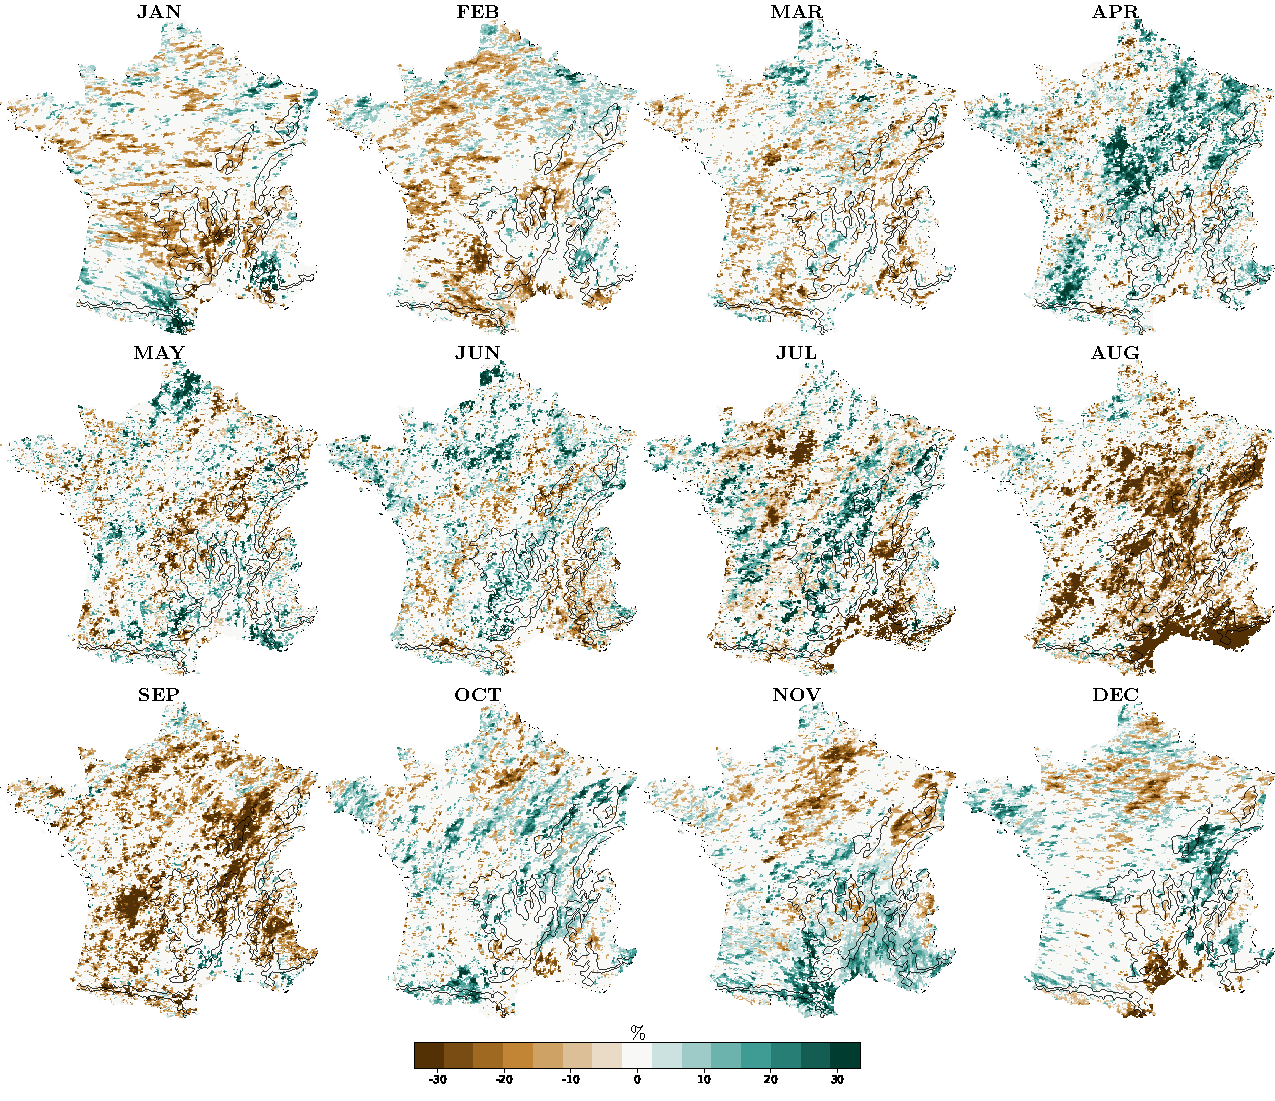
\includegraphics[width=\textwidth]{fig_AROME_trend_mois.pdf}
%    \\
%    \small FIGURE Z - Tendances horaires d'AROME sur la période 1959--2022 par mois.
%\end{figure}

\section{Discussion}\label{discussion}

\subsection{Climatology: consistencies, divergence and limitations}\label{climatology-consistencies-divergence-and-limitations}

The results confirm that AROME correctly reproduces the main rainfall
regimes over metropolitan France, as supported by the literature \parencites{Fumiere2020,Caillaud2021,hess-28-2579-2024,LucasPicher2024,Cortes-Hernandez2024}. It is able to reproduce the climatological orographic intensification of precipitation over the Alps,
the Pyrenees, and the Massif Central, a pronounced transition from Atlantic to continental climatic influence in the west, and the dryness of the Mediterranean
basin. This consistency with the stations indicates a satisfactory
representation of the dynamical forcings (moisture transport by westerly
flows, orographic uplift, low-level circulation in the Mediterranean).

AROME's ability to reproduce the frequency and quantity of precipitation and the 10-year return level of daily precipitation
is maintained throughout the year. Performance declines for the
10-year return level hourly precipitation specialy in summer.
The model underestimates high-intensity precipitation (\textgreater{} 40
mm/h \parencite{Caillaud2021,poncet2024convection}). Summer
convection remains partially under-resolved despite the 2.5 km spatial
resolution. In this study, we showed (results not shown) that
correlation increases (+30\%) when the time window is extended to 6 or 9 hours.
One can hypothesize that AROME spreads convective precipitation too widely in time and in space over nearby grid points, giving underestimated local peak precipitation. Unfortunately this hypothesis cannot be fully evaluated given the sparse station network. 
%The 2--3
%km grid spacing of AROME is a major step forward for representing convection
%without parameterization, but it remains too coarse for applications
%sensitive to intense maxima \parencite{prein2015regional}. 
A limitation of the evaluation performed in this study is indeed that it compares point-scale raingauge measurements with 2.5 km × 2.5 km AROME grid-box averages. This mismatch in spatial support is relatively modest for daily accumulations, but it becomes a major limitation at the hourly scale: a single convective core may affect only part of a grid cell, so that local station extremes can be much higher (or lower) than the corresponding AROME value even when the event is realistically simulated at the grid-box scale. A high-resolution gridded observational product would therefore be better suited to evaluating hourly extremes than individual stations. In this respect, Météo-France’s COMEPHORE product – a 1 km, hourly radar–gauge precipitation reanalysis over metropolitan France – would be particularly valuable \parencite{MeteoFrance_COMEPHORE_dataGouv}. It would have been interesting to include COMEPHORE in this study, but the reanalyses only begin in 1997, with poor quality over the Alps before 2007 \parencite{Fumiere2020}.

\subsection{Trends in precipitation extremes: consistencies,
divergences, and
limitations}\label{trends-in-precipitation-extremes-consistencies-divergences-and-limitations}

\subsubsection{Daily data: confirmation of known patterns and model–observation consistencies}

The daily trends derived from Météo-France stations confirm and refine previously documented spatial structures of extreme-precipitation evolution in France. The significant increases in the Rhône Valley and the southern Alps (+5 to +30\%) are fully consistent with earlier regional analyses reporting an intensification of daily extremes in southeastern France \parencites{Blanchet2018,blanchet2021explaining,Ribes2019}. The marked increases detected in northern France (locally up to +35\%) also agree with national-scale projections indicating a northward-shifted reinforcement of daily extremes under strong warming scenarios \parencite{soubeyroux:hal-04991790}. The weak or non-significant trends observed across large parts of western and central France likewise corroborate the high spatial variability highlighted in the IPCC report \parencite{IPCC2021}.

Overall, AROME reproduces the main spatial structures and magnitudes reasonably well when compared with the station-based climatology. The model correctly identifies regions of positive change (southern Alps, Rhône Valley, parts of northern France) and regions with weak or negative signals (western France, the Paris area), indicating an overall ability to capture the pattern of daily return-level evolution. However, AROME systematically underestimates the amplitude of the trends. This reduced magnitude is consistent with documented biases in the representation of extreme precipitation in AROME \parencite{caillaud2021simulation} and with the smoothing inherent to 2.5~km grid-box values.

\subsubsection{Hourly data: new national-scale findings and limited model–observation consistency}

Unlike the daily scale, no national mapping of hourly 10-year return-level trends has previously been available for France. The present work therefore provides the first nationwide characterization of hourly extreme-precipitation trends, offering new insight into their spatial organisation.

The station-based hourly trends exhibit far greater spatial heterogeneity and local variability than their daily counterparts. Over 1990–2022, trend magnitudes frequently reach $\pm 50\%$ and can exceed +100\%, with strong seasonal dependence. Coherent monthly signals emerge nonetheless: February trends in the Rhône Valley, March trends along the western Mediterranean arc, November increases in the eastern Mediterranean arc, and widespread June increases across most of France. These patterns, though noisier than daily trends, indicate that hourly extremes do exhibit structured temporal and spatial signatures, even within the constraints of a relatively short observational period.

AROME reproduces part of the structure of these hourly signals—particularly it concords in the months associated with enhanced extreme activity—but does not capture their spatial organization nor magnitude. Model–observation correlations remain low or near zero for most seasons and months, and the model substantially underestimates the amplitude of station-based trends. Even where stations show widespread enhancements (e.g.\ February, March, June), AROME simulates much weaker and spatially inconsistent changes. 
This limited agreement reflects the difficulty of reproducing localized convective extremes at 2.5~km resolution and the sensitivity of hourly diagnostics to spatial representativeness issues between point measurements and grid boxes.

Overall, the hourly results highlight two major conclusions: i) the station-derived hourly trends presented in this study constitute a new contribution to the climatology of French precipitation extremes, revealing structured yet highly localized patterns; ii) AROME currently shows limited skill in representing both the magnitude and spatial heterogeneity of hourly return-level trends, even when significant signals are isolated, underscoring the challenges of simulating sub-daily extremes.

%\subsection{Effect of record length on the detection of trends}
%Daily and hourly trends are estimated over different periods (1959--2022 for daily data, 1990--2022 for hourly data), which could suggest that the weaker and noisier hourly signals merely reflect the shorter hourly record. To assess this, we performed two complementary sensitivity checks (results not shown). First, when the daily analysis is restricted to 1990--2022, the spatial organisation and the sign of the 10-year return level trends remain very similar to those obtained over 1959--2022, with only a modest reduction in amplitude. This indicates that the main daily-scale signals identified in southeastern and northern France are not an artefact of the longer daily record. Second, AROME-only hourly trends computed over the full 1959--2022 simulation period (Figures~Y--Z) remain weak and spatially incoherent compared with the daily trends, even when the longer model record is used. Together, these sensitivity tests suggest that the contrast between well-structured daily trends and much less robust hourly trends is not solely due to differences in record length, but also reflects the greater intermittency of convective extremes and the current limitations of AROME in representing their temporal evolution at the hourly scale.


\section{Conclusion}\label{conclusion}

This study evaluated the ability of the convection-permitting regional climate model AROME (2.5\,km), forced by ERA5 over 1959--2022, to reproduce the climatology and the recent evolution of extreme precipitation in metropolitan France, using Météo-France rain-gauge observations at daily (1959--2022) and hourly (1990--2022) time scales. Extremes were characterized with EVT using GEV models (stationary and non-stationary), and trends were quantified through changes in 10-year return levels.

%At the climatological level, AROME reproduces the main spatial structures of precipitation over France, including the strong orographic enhancement over mountain ranges and the dry Mediterranean coastal belt. Agreement with station-based indicators is very high for precipitation frequency and annual totals, and remains high for daily 10-year return levels. Spatially coherent biases persist, with localized overestimation in some mountainous regions and underestimation in several coastal and foothill areas. At the hourly scale, the model shows a systematic negative bias in the 10-year return level and a strong degradation of spatial correlations in summer, consistent with an under-representation of intense convective peaks and with timing and localization errors that have a limited impact on daily accumulations but a strong impact on hourly diagnostics.

%For daily extremes, station-based trends in 10-year return levels show structured, region-dependent signals over 1959--2022, with the most robust increases in the South-Eastern Alps and a reinforcement along the Rhône Valley, while large parts of western and central France exhibit weak or non-significant trends. AROME generally captures the large-scale sign and organization of these daily trend patterns, indicating that the simulation contains relevant information on the spatial structure of changes in daily extremes. However, trend amplitudes are usually weaker in the model than in the observations. This attenuation is consistent with the grid-box smoothing at 2.5\,km, with known biases in AROME for high-intensity precipitation, and with the reported underestimation of temperature trends in the ERA5-forced configuration, which likely reduces the thermodynamic contribution to changes in extreme precipitation.

%For hourly extremes, the station-based trends derived over 1990--2022 are much more heterogeneous and locally extreme than at the daily scale, reflecting both the intrinsic intermittency of convective precipitation and the limited length of hourly records. Despite this noise, the monthly analysis reveals recurrent windows of enhanced change (notably in late winter, early spring, late autumn, and June), suggesting that hourly extremes can exhibit seasonally concentrated signals rather than uniform annual changes. AROME captures part of the timing of these monthly windows but shows limited skill in reproducing the spatial organization and the magnitude of hourly return-level trends, with correlations close to zero for several seasons and months. These results highlight that, at 2.5\,km resolution, the representation of the temporal evolution of highly localized convective extremes remains challenging, and that point-to-grid representativeness issues strongly limit model--station consistency at the hourly scale.

Overall, the AROME model provides clear added value for the climatology and the spatial organization of daily extremes, and it can support national-scale analyses of daily extreme-precipitation changes, provided that trend magnitudes are interpreted cautiously. In contrast, the evaluation indicates that hourly return levels and especially their trends are less well reproduced, with hourly trends almost inexistent in AROME. However our evaluation shows limitation at hourly scale due to spatial support mismatch between stations and grid points, and short observational record length of stations that prevented us from making the comparison at hourly scale over the full 1959--2022 simulation period. Future work should rely on high-resolution gridded reference datasets (e.g.\ radar--gauge reanalyses) to reduce representativeness errors, investigate the sensitivity of results to temporal aggregation (multi-hour maxima, intensity-duration-frequency curves), and exploit the full 1959--2022 AROME record to explore the emergence of signals beyond the short observational hourly period. These steps are needed to better constrain sub-daily extreme precipitation changes relevant to flash-flood hazard in France.

\section*{References}\label{references}
\printbibliography[heading=none]
%\bibliographystyle{apalike}
%\bibliography{references}

\end{document}